\chapter{The Game}\label{ch:game}

\begin{center}
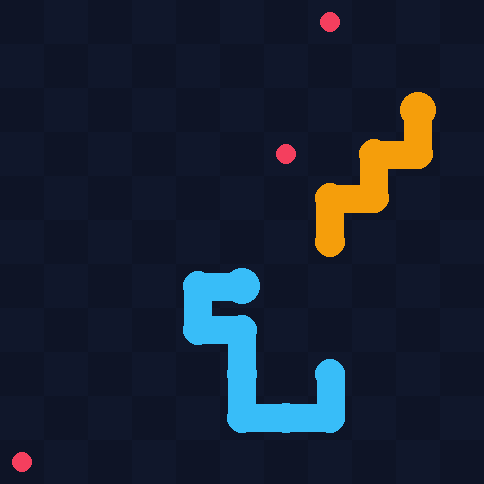
\includegraphics[width=0.46\linewidth]{figures/duel_board.png}
\captionof{figure}{A duel at turn 45, both seats played by the trained network. Heads
are the larger discs; red dots are food.}
\label{fig:duel-board}
\end{center}

\section{The board and the snakes}

\begin{defbox}[Game state]
A game is played on a $B\times B$ grid of cells $(r,c)$, row $0$ at the top, with
$B\ge 7$ ($B=11$ by default). It has $S\in\{1,\dots,8\}$ snakes. Snake $k$ has
\begin{itemize}
\item a \emph{body} $\bigl(x^k_0, x^k_1, \dots, x^k_{L_k-1}\bigr)$, a list of cells with the head
  $x^k_0$ first. Cells may repeat; this matters, see below.
\item a \emph{length} $L_k$, the number of entries in the body;
\item a \emph{health} $h_k \in \{0,\dots,h_{\max}\}$ with $h_{\max}=100$;
\item an \emph{alive} flag.
\end{itemize}
The board also holds a set of food cells $F$, a turn counter, and the game's
\emph{minimum food} $f_{\min}$, which is $1$ in standard play.
\end{defbox}

\textbf{Actions.} Every turn each living snake chooses one of four absolute directions,
$a\in\{\uparrow,\downarrow,\leftarrow,\rightarrow\}$, encoded $0$--$3$. All snakes move
\emph{simultaneously}; nobody sees the others' choices before committing. Reversing onto
your own neck is legal but fatal, exactly as in the official game.

\section{One turn}

\begin{algbox}[Turn order (Battlesnake standard)]
Given every snake's action:
\begin{enumerate}
\item \textbf{Move.} Each living snake's body becomes $\bigl(x_0 + \delta(a),\ x_0,\ \dots,\ x_{L-2}\bigr)$:
  a new head is added and the last segment drops off.
\item \textbf{Health.} Every moving snake loses one health point.
\item \textbf{Feed.} A snake whose new head is on food resets its health to $h_{\max}$
  and \emph{duplicates its last segment}, so its length grows by one. The food is removed
  after all snakes have fed, so two heads on one food both eat.
\item \textbf{Spawn food.} If $|F| < f_{\min}$, or with probability $15\%$ otherwise, one
  food appears on a uniformly random free cell.
\item \textbf{Eliminate.} First remove every snake that starved ($h\le 0$) or left the
  board. Then, simultaneously among the rest, a snake is eliminated if its head lies on
  any body segment other than a head (its own included), or if it meets another head
  whose snake is \emph{at least as long}.
\item \textbf{End.} With $S>1$ the game ends when at most one snake is alive; the
  survivor, if any, wins. A single snake's game ends when it dies.
\end{enumerate}
\end{algbox}

\begin{warnbox}[Growth is a duplicated tail, not an extra head]
When a snake eats, its tail stays put \emph{on the next turn}, because the duplicated
segment is what drops off. Two consequences follow, and both are easy to get wrong:
\begin{itemize}
\item moving into a cell that an opponent's tail is vacating is \emph{safe}, unless that
  opponent ate last turn, in which case the tail does not move and the move is fatal;
\item a snake's length counts the duplicate. A snake that fills all $64$ cells of an
  $8\times8$ board by eating the food spawned into its own vacated tail cell ends with
  length $65$, not $64$. This was caught by a test (Chapter~\ref{ch:baselines}).
\end{itemize}
\end{warnbox}

\section{Head-to-head collisions}

The head-to-head rule is what makes the game strategic rather than a race to eat. Let
$P_k$ be the cell snake $k$ moves into. Snake $k$ is eliminated by a head-to-head if
\[
  \exists\, j\ne k:\quad P_j = P_k \ \text{ and }\ L_j \ge L_k .
\]
Equal lengths eliminate \emph{both} snakes. Being longer therefore makes a snake a
threat to every neighbouring head, and this is exactly what one of the observation
planes encodes (Chapter~\ref{ch:obs}).

\section{Setup}

\begin{defbox}[Start positions and initial food]
Let $a=1$, $m=\lfloor B/2\rfloor$, $z=B-2$. The eight start cells are the four
\emph{corners} $\{(a,a),(a,z),(z,a),(z,z)\}$ and the four \emph{edge midpoints}
$\{(a,m),(m,a),(m,z),(z,m)\}$. Each game picks one group with probability $\tfrac12$ and
fills it first, in random order, so with $S\le4$ snakes all start equidistant from the
centre. Every snake starts with length $3$, all three segments stacked on its start cell.

Food is placed on the centre cell, and for each snake on one of its four diagonal
neighbours, chosen uniformly among those that are not a board corner and are not
strictly closer to the centre than the snake itself.
\end{defbox}

\section{As a Markov game}

For learning, the game is a stochastic game with $S$ players. The state is
the full board; the transition is the turn order above, whose only randomness is food
spawning; and each player's reward is
\[
  R_k \;=\;
  \begin{cases}
    +1 & \text{if } k \text{ is the last snake alive,}\\
    -1 & \text{on the turn } k \text{ is eliminated, unless every remaining snake falls on that turn,}\\
    \hphantom{+}0 & \text{otherwise.}
  \end{cases}
\]
A turn on which the last snakes all fall together is a \emph{draw}, worth $0$ to each of
them. Each player observes the board from its own point of view (Chapter~\ref{ch:obs}).
Because every seat runs the same rules and sees an egocentric view, a single policy
network can play every seat at once, which is what self-play exploits.
